\documentclass[a4paper,10pt,oneside,final,titlepage,onecolumn]{article}

\usepackage{ucs}
\usepackage[portuguese]{babel}
\usepackage[utf8x]{inputenc}
\usepackage[T1]{fontenc}
\usepackage{textcomp}
\usepackage{graphicx}
\usepackage{placeins}

\usepackage{listings}
\usepackage{color}

\definecolor{dkgreen}{rgb}{0,0.6,0}
\definecolor{gray}{rgb}{0.5,0.5,0.5}
\definecolor{mauve}{rgb}{0.58,0,0.82}

\lstset{frame=tb,
  language=bash,
  aboveskip=3mm,
  belowskip=3mm,
  showstringspaces=false,
  columns=flexible,
  basicstyle={\scriptsize\ttfamily},
  numbers=none,  
  breaklines=true,
  breakatwhitespace=true
  tabsize=3
}



\title{Exercício 3 de MC833 --- Programação em Redes de Computadores}
\author{Raul Rabelo Carvalho, 105607, turma A}



\begin{document}



\maketitle



\section{htons}
\paragraph{}A função \verb|htons| faz parte de um conjunto de funções usadas para converter um inteiro, tanto de 16 bits quanto de 32 bits, entre a \emph{byte order} de rede (\emph{big endian}) e a \emph{byte order} do \emph{host} local, que pode ser \emph{big endian} ou \emph{little endian} a depender da arquitetura. É óbvio que caso a arquitetura do \emph{host} seja \emph{big endian}, nada é feito.
\paragraph{}Especificamente, a função \verb|htons| converte inteiros de 16 bits da \emph{byte order} do \emph{host} para da rede.



\FloatBarrier
\section{Execução com código-fonte não-modificado}
\paragraph{}Não é possível executar o servidor sem alterações no \emph{host} do laboratório do IC (\verb|guns.ic.unicamp.br|), pois a função \verb|bind| não tem permissão para utilizar a porta 10. Esta porta é uma das \emph{well-known ports} e estão bloqueadas para usuários sem privilégios nas máquinas do IC.



\FloatBarrier
\section{Resolvendo o problema do bind}
\paragraph{}Alterando-se a porta empregada para 1234, tanto em \verb|client.c| quanto em \verb|server.c|, resolve-se o problema do servidor não conseguir reservar para si uma das \emph{well-known ports}. No entanto, o cliente não consegue se conectar a esta porta, provavelmente devido àlguma política de bloqueio de portas no roteador dos laboratórios.
\paragraph{}Fazendo uma segunda alteração para a porta 10000, o servidor consegue reservar a porta e executar normalmente, e o cliente consegue conectar-se a esta porta e comunicar-se com o servidor, como na figura \ref{exec-local}.
\begin{figure}[!ht]
  \caption{Execução local.}
  \centering
  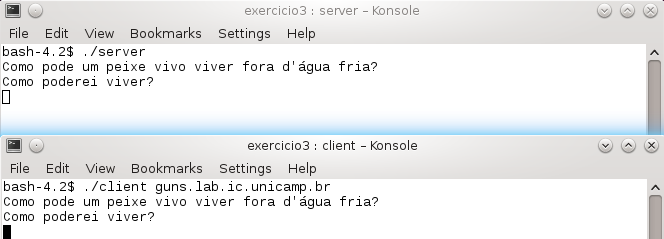
\includegraphics[width=117mm]{images/exec-local.png}
  \label{exec-local}
\end{figure}
\paragraph{}Também foi possível executar o servidor no \emph{host} local e o cliente na máquina \verb|xaveco| via \verb|ssh|, executado com o comando \verb|./client guns.lab.ic.unicamp.br|.
\begin{figure}[!ht]
  \caption{Execução remota.}
  \centering
  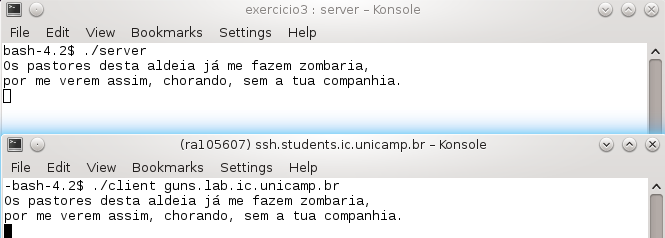
\includegraphics[width=117mm]{images/exec-remota.png}
  \label{exec-remota}
\end{figure}



\FloatBarrier
\section{Múltiplos clientes}
\paragraph{}O comportamento dos clientes e do servidor quando dez clientes tentam se conectar ao servidor, quando este está configurado com um \emph{backlog} de cinco está mostrado nas figuras \ref{multiplos1}, \ref{multiplos2} e \ref{multiplos3}. O que ocorre é que além do primeiro cliente cuja conexão foi aceita, mais seis conexões foram sendo aceitas a medida em que as anteriores eram encerradas. A sexta conexão além das cinco em que o servidor configurou o \verb|socket| pode ser devido à implementação deste no sistema, pois a maioria dos sistemas operacionais tomam o parâmetro \emph{backlog} como uma indicação e não como uma regra forte a ser seguida\footnote{Stevens, Fenner, Rudoff, "Unix Network Programming: The Sockets Network API", Volume 1, Third Edition, pp. 106-108.}
\begin{figure}[!ht]
  \caption{Servidor com backlog de 5 e dez clientes conectados.}
  \centering
  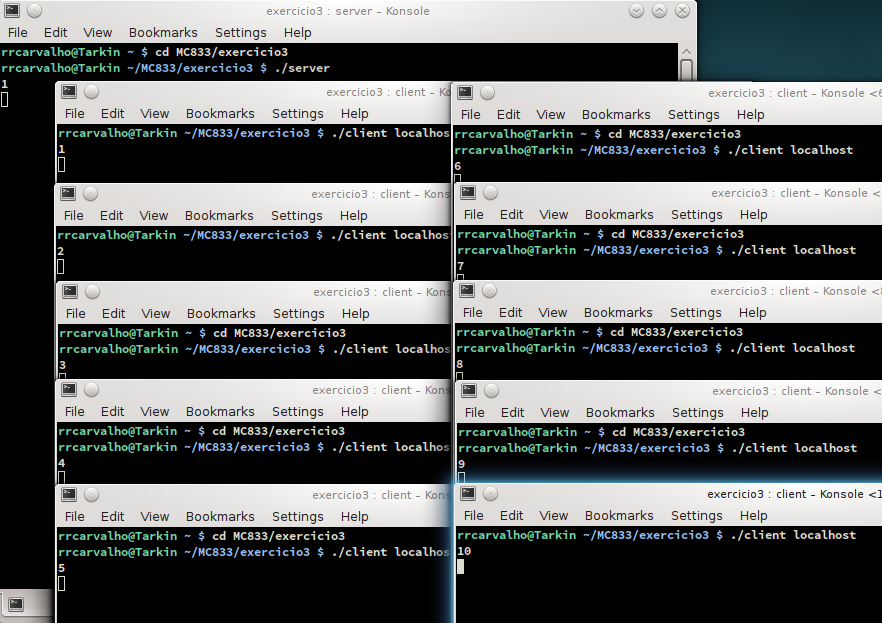
\includegraphics[width=117mm]{images/multiplos1.png}
  \label{multiplos1}
\end{figure}
\begin{figure}[!ht]
  \caption{Servidor com backlog de 5 após o encerramento do primeiro dos dez clientes.}
  \centering
  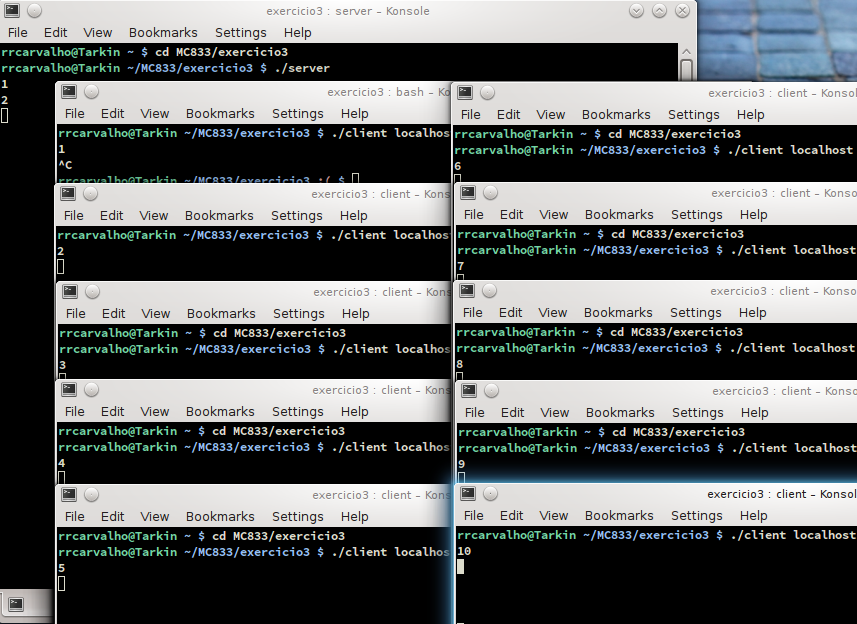
\includegraphics[width=117mm]{images/multiplos2.png}
  \label{multiplos2}
\end{figure}
\begin{figure}[!ht]
  \caption{Servidor com backlog de 5 após o encerramento dos dez clientes.}
  \centering
  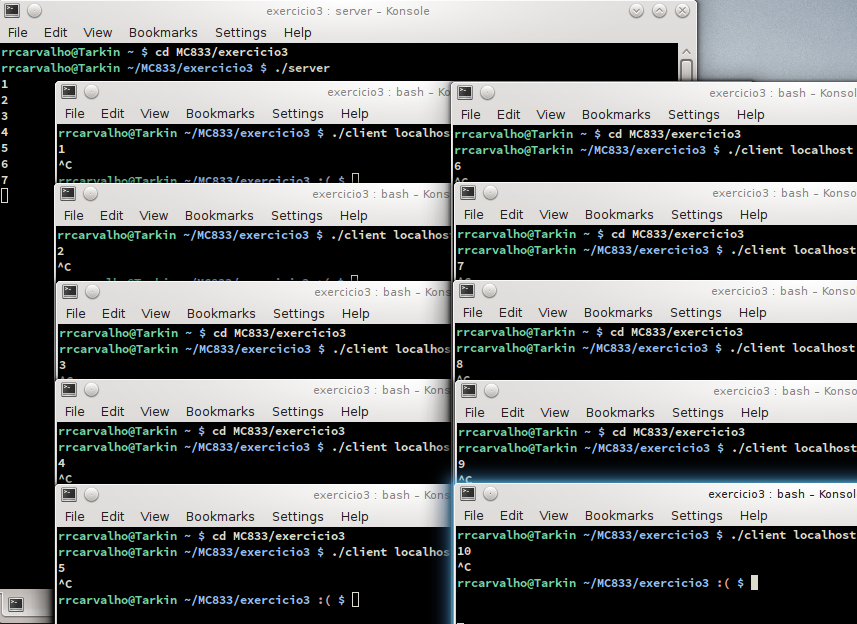
\includegraphics[width=117mm]{images/multiplos3.png}
  \label{multiplos3}
\end{figure}
\paragraph{}O \emph{backlog} do servidor foi mudado para um e o resultado de dez conexões é mostrado nas figuras \ref{multiplos4}, \ref{multiplos5} e \ref{multiplos6}. Ocorre novamente que um cliente extra além do cliente 2 que estava na fila de tamanho um agora conseguiu se conectar; e, além disso, o cliente 10 também se conectou logo após o cliente 3 ser encerrado. Ocorre que o tempo gasto na obtenção das imagens não foi longo o suficiente para o \emph{timeout} do cliente 10 ter se esgotado quando do encerramento do cliente 2, assim, ele foi capaz de entrar na fila tão logo o cliente 1 foi encerrado. Aguardando um tempo maior antes de encerrar as conexões (figura \ref{multiplos7}, o cliente 10 não consegue uma conexão.
\begin{figure}[!ht]
  \caption{Servidor com backlog de 1 e dez clientes conectados.}
  \centering
  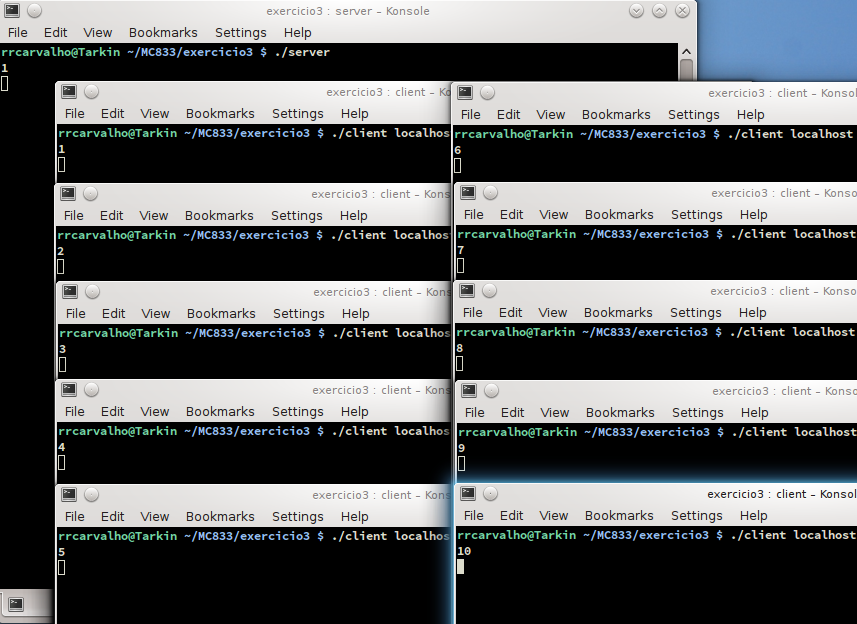
\includegraphics[width=117mm]{images/multiplos4.png}
  \label{multiplos4}
\end{figure}
\begin{figure}[!ht]
  \caption{Servidor com backlog de 1 após o encerramento do primeiro dos dez clientes.}
  \centering
  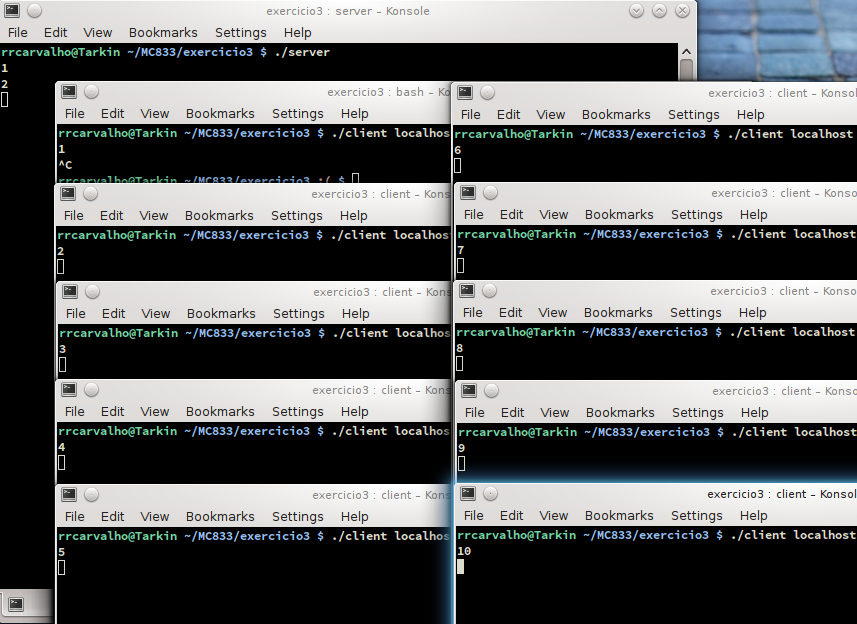
\includegraphics[width=117mm]{images/multiplos5.png}
  \label{multiplos5}
\end{figure}
\begin{figure}[!ht]
  \caption{Servidor com backlog de 1 após o encerramento dos dez clientes.}
  \centering
  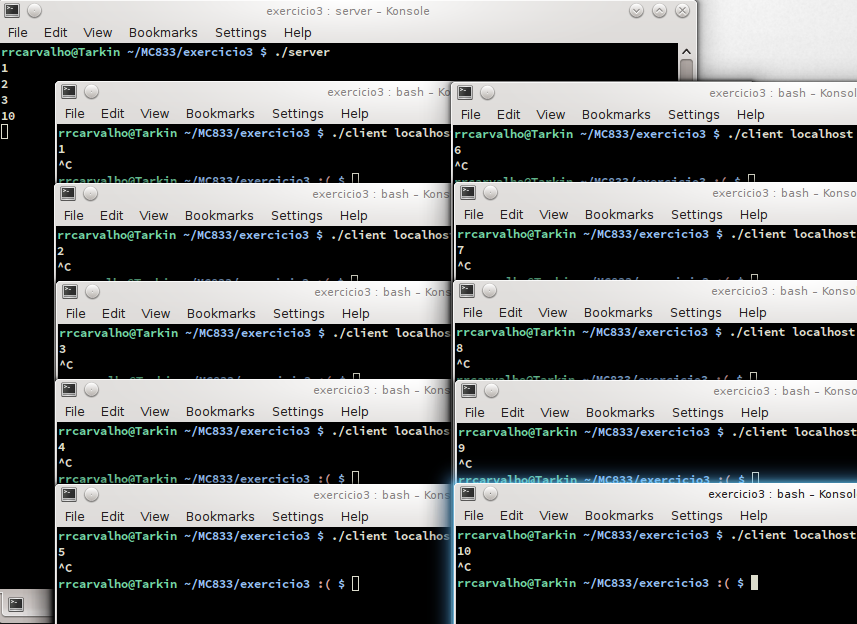
\includegraphics[width=117mm]{images/multiplos6.png}
  \label{multiplos6}
\end{figure}
\begin{figure}[!ht]
  \caption{Servidor com backlog de 1 com os 10 clientes encerrados depois de vários minutos.}
  \centering
  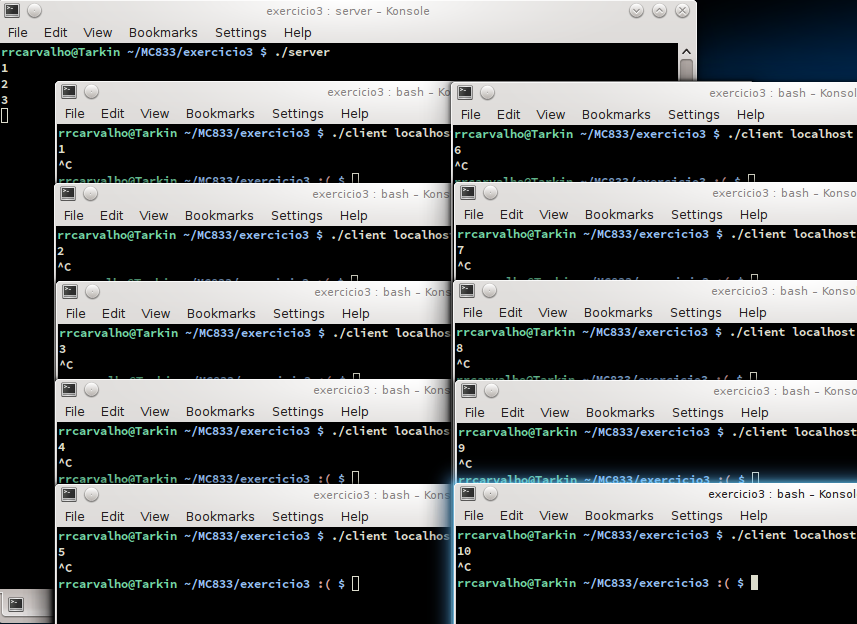
\includegraphics[width=117mm]{images/multiplos7.png}
  \label{multiplos7}
\end{figure}



\FloatBarrier
\section{Verificando o uso da rede}
\paragraph{}Pode-se configurar a porta usada no servidor para uma porta disponível no \emph{host} em que ele vá ser executado. Com conhecimento desta porta, se estabelece a conexão entre cliente e servidor normalmente. Em um terceiro \verb|terminal|, executa-se o comando \verb|netstat -tu| e, se a comunicaçao entre cliente e servidor se faz por rede, uma conexão estabelecida com endereço IP do \emph{host} do servidor e a porta TCP empregada estará listada na saída desta ferramenta.
\paragraph{}Como mostrado na figura \ref{netstat}, existe uma conexão estabelecida entre o servidor em \verb|xaveco.lab.ic.unicamp.br|, usando a porta 10101. Foi usado o comando \verb|netstat -tun|, pois a porta 10101, apesar de estar acima de 1024, tem uma aplicação conhecida associada a ela. A conexão em questão está listada na terceira linha da saída do comando \verb|netstat| e um \emph{reverse} \verb|nslookup| foi feito para se confirmar que o endereço IP \verb|143.106.16.163| corresponde ao nome \verb|xaveco.lab.ic.unicamp.br|.
\begin{figure}[!ht]
  \caption{Netstat -tun.}
  \centering
  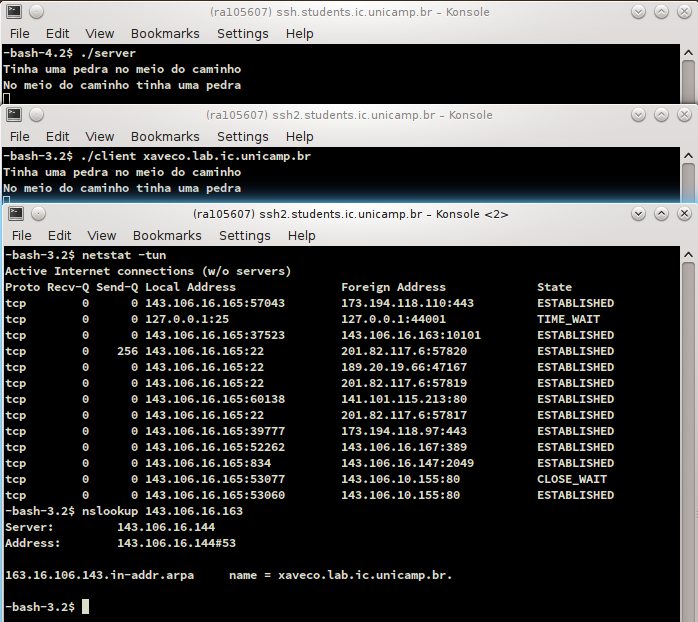
\includegraphics[width=117mm]{images/netstat.png}
  \label{netstat}
\end{figure}



\FloatBarrier
\section{telnet}
\paragraph{}A figura \ref{telnet} mostra o programa \verb|telnet| conectando-se e enviando mensagens ao servidor. Como o \verb|telnet| usa o protocolo TCP e pode conectar-se a qualquer porta, não só a porta 23 do protocolo Telnet, um modo de impedir o acesso ao servidor é modificá-lo para receber pacotes UDP, o que implicaria em uma mudança no cliente também.
\begin{figure}[!ht]
  \caption{Usando telnet como cliente.}
  \centering
  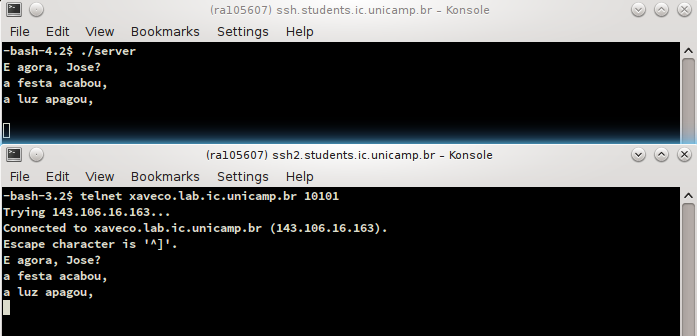
\includegraphics[width=117mm]{images/telnet.png}
  \label{telnet}
\end{figure}



\FloatBarrier
\section{echo}
\paragraph{}Para a implementação da funcionalidade de \emph{echo} no cliente e no servidor, foram modificadas algumas linhas no \emph{loop} principal dos programas. Em \verb|client.c|:
\begin{lstlisting}
	while (fgets(buf, sizeof(buf), stdin)) {
		buf[MAX_LINE-1] = '\0';
		len = strlen(buf) + 1;
		send(s, buf, len, 0);
		while (len = recv(s, buf, sizeof(buf), 0)) {
			fputs(buf, stdout);
			if (len) break;
		}
	}
\end{lstlisting}
\paragraph{}E em \verb|server.c|:
\begin{lstlisting}
	while(1) {
		if ((new_s = accept(s, (struct sockaddr *)&sin, &len)) < 0) {
			perror("simplex-talk: accept");
			exit(1);
		}
		while (len = recv(new_s, buf, sizeof(buf), 0)) {
			fputs(buf, stdout);
			send(new_s, buf, len, 0);
		}
		close(new_s);
	}
\end{lstlisting}
A figura \ref{echo} mostra a saída dos programas modificados.
\begin{figure}[!ht]
  \caption{Echo no cliente da linha transmitida.}
  \centering
  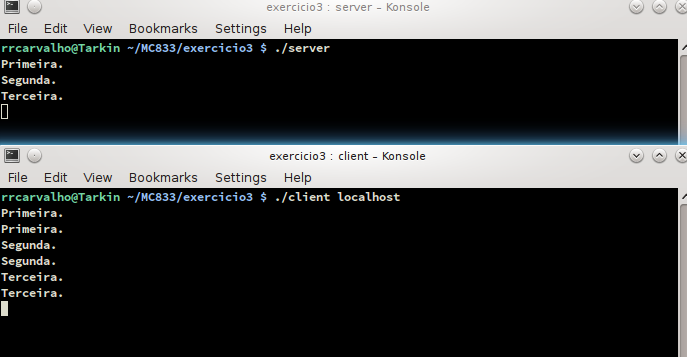
\includegraphics[width=117mm]{images/echo.png}
  \label{echo}
\end{figure}

\end{document}
